\documentclass{article}
\usepackage{graphicx} %for inserting image

\title{Software Requirements Document : Tetris Royal}
\author{Tao Chau\\
		Juliete Cornu-Besser\\
		Quentin Bernard Bouissières\\
		Jonas Schellekens\\
		Ethan Van Ruyskenvelde\\
		Lucas Verbeiren\\
		Ernerst Malysz\\
		Rafaou Gajewicz}

\date{ 13 décembre 2024}

\begin{document}
\maketitle

\newpage

\tableofcontents

\newpage

\section{Introduction}

\subsection{But du projet}

\quad L'objectif de ce projet est d'implémenter une application jeu avec une option multijoueur. Les règles des parties reprendront celles existantes dans \textit{Tetris Royal}, une extension de la version normale. Chaque joueur possède une grille vide qu'il doit essayer de remplir en laissant le moins d'espace possible avec des \textit{tetriminos}, des formes géométriques avec une possibilité au joeur de les tourner et les déplacer, qui "tombent d'en haut" de la grille. Une ligne remplie de  \textit{tetriminos} se supprime et fait gagner des points au joueur. La partie se termine quand le joueur ne sait plus placer de formes géométriques sur la grille; son score dépendra du temps et des lignes supprimées.  %j'aime absolument pas cette formulation
\\ \\
\quad Dans cette application, quatre modes sont proposés au joueur. Il existe la version \textit{Endless} avec un seul joueur où le but est de savoir placer des pièces sur la grille le plus longtemps possible. Selon les combinaisons des pièces qui se suppriment, les points attribués seront différemment. 
% je n'aime pas cette formulation
Puis nous implémentons les modes multijoueurs. Une nouvelle notion doit être introduite : "\textit{une ligne de malus}". Un joueur peut envoyer un malus à un adversaire. Le receveur du malus a toutes ses lignes poussées vers le haut d'une ligne ou plus pour laisser la place à une ou plusieurs rangées avec un bloc manquant en dessous.  La version \textit{Classic} et celle \textit{Duel} comprennent des parties de trois à neuf et deux joueurs respectivement. Chaque participant a sa propre grille avec ses \textit{tetriminos} qui tombent du haut de la grille; celui qui complète une ligne ou plusieurs lignes en même temps, il peut envoyer des lignes de malus selon sa combinaison à un adversaire de son choix. Le dernier mode, \textit{ Royal Competition}, comprend des malus et des bonus. 
\subsection{Glossaire}

\subsection{Historique}

\section{Besoins utilisateurs}

\subsection{Écran d'accueil}

\subsubsection{Inscription}

\subsubsection{Connexion}

\begin{figure}
    \centering
    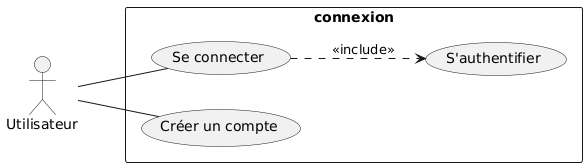
\includegraphics[width=0.9\textwidth]{./uml/usescase/connexion/connexion.png}
    \caption{Diagramme Use Case du Menu Principal}
    \label{fig:main-menu}
\end{figure}

\subsection*{Se connecter}
\begin{itemize}
    \item \textbf{Acteur}: Utilisateur
    \item \textbf{Use case}: Se connecter
    \item \textbf{Description}: Permet à l'utilisateur de se connecter au système.
    \item \textbf{Précondition}: L'utilisateur possède déjà un compte.
    \item \textbf{Postcondition}: L'utilisateur est connecté au système.
    \item \textbf{Cas exceptionnels}: Mauvais identifiant ou mot de passe, échec de la connexion réseau.
\end{itemize}

\subsection*{Créer un compte}
\begin{itemize}
    \item \textbf{Acteur}: Utilisateur
    \item \textbf{Use case}: Créer un compte
    \item \textbf{Description}: Permet à un utilisateur de s’inscrire et de créer un compte.
    \item \textbf{Précondition}: L’utilisateur n’a pas encore de compte.
    \item \textbf{Postcondition}: Un nouveau compte est créé et l'utilisateur est authentifié.
    \item \textbf{Cas exceptionnels}: L'utilisateur existe déjà, erreurs de validation de données.
\end{itemize}

\subsection*{S'authentifier}
\begin{itemize}
    \item \textbf{Acteur}: Utilisateur
    \item \textbf{Use case}: S'authentifier
    \item \textbf{Description}: Vérifie les informations d'identification fournies par l'utilisateur.
    \item \textbf{Précondition}: L'utilisateur a soumis ses identifiants.
    \item \textbf{Postcondition}: Authentification réussie, session utilisateur créée.
    \item \textbf{Cas exceptionnels}: Identifiants incorrects, serveur d’authentification indisponible.
\end{itemize}
\newpage

\subsection{Menu Principal}

\begin{figure}
    \centering
    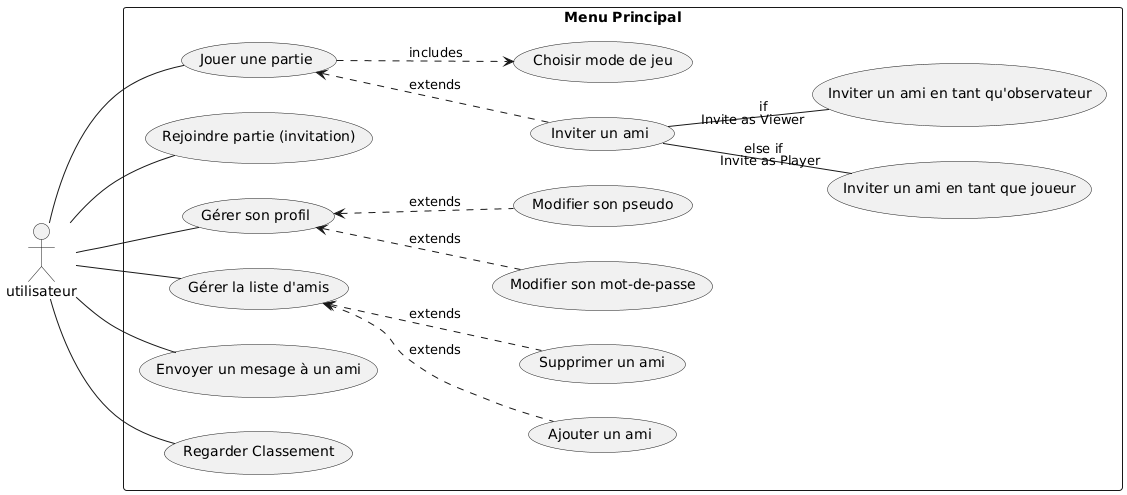
\includegraphics[width=0.9\textwidth]{./uml/usescase/menu-principal/menu_principal.png}
    \caption{Diagramme Use Case du Menu Principal}
    \label{fig:main-menu}
\end{figure}

\subsubsection*{Jouer une partie}
\begin{itemize}
    \item \textbf{Acteur}: Utilisateur
    \item \textbf{Use case}: Jouer une partie
    \item \textbf{Description}: Permet à l'utilisateur de lancer une partie.
    \item \textbf{Précondition}: L'utilisateur est authentifié.
    \item \textbf{Postcondition}: Une partie de jeu est démarrée.
    \item \textbf{Cas exceptionnels}: Problème de connexion ou erreurs de lancement.
\end{itemize}

\subsubsection*{Rejoindre partie (invitation)}
\begin{itemize}
    \item \textbf{Acteur}: Utilisateur
    \item \textbf{Use case}: Rejoindre partie (invitation)
    \item \textbf{Description}: Permet à l'utilisateur de rejoindre une partie sur invitation d'un ami.
    \item \textbf{Précondition}: L'utilisateur a reçu une invitation.
    \item \textbf{Postcondition}: L'utilisateur rejoint la partie.
    \item \textbf{Cas exceptionnels}: Invitation expirée, partie pleine.
\end{itemize}

\subsubsection*{Inviter un ami}
\begin{itemize}
    \item \textbf{Acteur}: Utilisateur
    \item \textbf{Use case}: Inviter un ami
    \item \textbf{Description}: Permet à l'utilisateur d'inviter un ami à une partie.
    \item \textbf{Précondition}: L'ami est connecté.
    \item \textbf{Postcondition}: Invitation envoyée à l'ami.
    \item \textbf{Cas exceptionnels}: L'ami est indisponible ou n'accepte pas l'invitation.
\end{itemize}

\subsubsection*{Choisir mode de jeu}
\begin{itemize}
    \item \textbf{Acteur}: Utilisateur
    \item \textbf{Use case}: Choisir mode de jeu
    \item \textbf{Description}: Permet à l'utilisateur de choisir le mode de jeu.
    \item \textbf{Précondition}: Une partie est sur le point de commencer.
    \item \textbf{Postcondition}: Le mode de jeu est défini pour la partie.
    \item \textbf{Cas exceptionnels}: Mode de jeu non disponible.
\end{itemize}

\subsubsection*{Gérer son profil}
\begin{itemize}
    \item \textbf{Acteur}: Utilisateur
    \item \textbf{Use case}: Gérer son profil
    \item \textbf{Description}: Permet à l'utilisateur de modifier les informations de son profil.
    \item \textbf{Précondition}: L'utilisateur est authentifié.
    \item \textbf{Postcondition}: Les informations de profil sont mises à jour.
    \item \textbf{Cas exceptionnels}: Échec de la mise à jour des informations.
\end{itemize}

\subsubsection*{Gérer la liste d'amis}
\begin{itemize}
    \item \textbf{Acteur}: Utilisateur
    \item \textbf{Use case}: Gérer la liste d'amis
    \item \textbf{Description}: Permet à l'utilisateur de gérer sa liste d'amis.
    \item \textbf{Précondition}: L'utilisateur est connecté.
    \item \textbf{Postcondition}: La liste d'amis est mise à jour.
    \item \textbf{Cas exceptionnels}: Problèmes de synchronisation, ami introuvable.
\end{itemize}

\subsubsection*{Envoyer un message à un ami}
\begin{itemize}
    \item \textbf{Acteur}: Utilisateur
    \item \textbf{Use case}: Envoyer un message à un ami
    \item \textbf{Description}: Permet à l'utilisateur d'envoyer un message à un ami.
    \item \textbf{Précondition}: L'ami est dans la liste d'amis.
    \item \textbf{Postcondition}: Le message est envoyé avec succès.
    \item \textbf{Cas exceptionnels}: Ami déconnecté ou problème de réseau.
\end{itemize}

\subsubsection*{Modifier son mot-de-passe}
\begin{itemize}
    \item \textbf{Acteur}: Utilisateur
    \item \textbf{Use case}: Modifier son mot-de-passe
    \item \textbf{Description}: Permet à l'utilisateur de changer son mot de passe.
    \item \textbf{Précondition}: L'utilisateur est authentifié.
    \item \textbf{Postcondition}: Le mot de passe est modifié avec succès.
    \item \textbf{Cas exceptionnels}: Mot de passe actuel incorrect, validation échouée.
\end{itemize}

\subsubsection*{Modifier son pseudo}
\begin{itemize}
    \item \textbf{Acteur}: Utilisateur
    \item \textbf{Use case}: Modifier son pseudo
    \item \textbf{Description}: Permet à l'utilisateur de changer son pseudo.
    \item \textbf{Précondition}: L'utilisateur est authentifié.
    \item \textbf{Postcondition}: Le pseudo est modifié avec succès.
    \item \textbf{Cas exceptionnels}: Pseudo déjà pris, validation échouée.
\end{itemize}

\subsubsection*{Ajouter un ami}
\begin{itemize}
    \item \textbf{Acteur}: Utilisateur
    \item \textbf{Use case}: Ajouter un ami
    \item \textbf{Description}: Permet à l'utilisateur d'ajouter un autre utilisateur à sa liste d'amis.
    \item \textbf{Précondition}: L'autre utilisateur existe et est accessible.
    \item \textbf{Postcondition}: L'utilisateur est ajouté en tant qu'ami.
    \item \textbf{Cas exceptionnels}: Ami déjà présent dans la liste, utilisateur introuvable.
\end{itemize}

\subsubsection*{Supprimer un ami}
\begin{itemize}
    \item \textbf{Acteur}: Utilisateur
    \item \textbf{Use case}: Supprimer un ami
    \item \textbf{Description}: Permet à l'utilisateur de retirer un ami de sa liste.
    \item \textbf{Précondition}: L'ami existe dans la liste d'amis.
    \item \textbf{Postcondition}: L'ami est supprimé de la liste.
    \item \textbf{Cas exceptionnels}: L'ami n'est plus dans la liste ou une erreur de suppression.
\end{itemize}

\subsubsection*{Inviter un ami en tant que joueur}
\begin{itemize}
    \item \textbf{Acteur}: Utilisateur
    \item \textbf{Use case}: Inviter un ami en tant que joueur
    \item \textbf{Description}: Permet à l'utilisateur d'inviter un ami pour participer à une partie.
    \item \textbf{Précondition}: L'ami est connecté.
    \item \textbf{Postcondition}: Invitation envoyée pour jouer.
    \item \textbf{Cas exceptionnels}: L'ami n'est pas disponible, invitation rejetée.
\end{itemize}

\subsubsection*{Inviter un ami en tant qu'observateur}
\begin{itemize}
    \item \textbf{Acteur}: Utilisateur
    \item \textbf{Use case}: Inviter un ami en tant qu'observateur
    \item \textbf{Description}: Permet à l'utilisateur d'inviter un ami pour observer une partie.
    \item \textbf{Précondition}: L'ami est connecté.
    \item \textbf{Postcondition}: Invitation envoyée pour observer.
    \item \textbf{Cas exceptionnels}: L'ami est indisponible, invitation rejetée.
\end{itemize}

\subsubsection*{Regarder Classement}
\begin{itemize}
    \item \textbf{Acteur}: Utilisateur
    \item \textbf{Use case}: Regarder Classement
    \item \textbf{Description}: Permet à l'utilisateur de consulter les classements.
    \item \textbf{Précondition}: L'utilisateur est connecté.
    \item \textbf{Postcondition}: Le classement est affiché.
    \item \textbf{Cas exceptionnels}: Classement indisponible.
\end{itemize}

\subsubsection{Lancer une partie}

\subsubsection{Amis}

\subsubsection{Chat hors partie}

\subsubsection{Affichage du classement}

\subsection{Lancement d'une partie}

\subsubsection{Créer une partie}

\subsubsection{Rejoindre une partie}

\begin{figure}
    \centering
    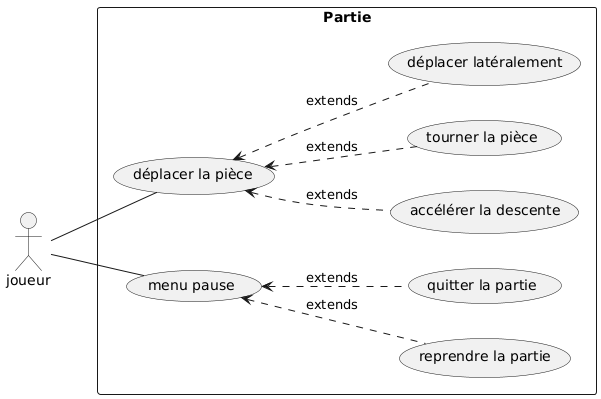
\includegraphics[width=0.9\textwidth]{./uml/usescase/en-jeu/endless.png}
    \caption{Diagramme Use Case en mode Classique}
    \label{fig:Classique}
\end{figure}

\begin{itemize}
    \item \textbf{Acteur}
    \item \textbf{Use case}
    \item \textbf{Description}
    \item \textbf{Précondition}
    \item \textbf{Postcondition}
    \item \textbf{Cas exceptionnels}
\end{itemize}

\subsubsection{En partie Duel}

\begin{figure}
    \centering
    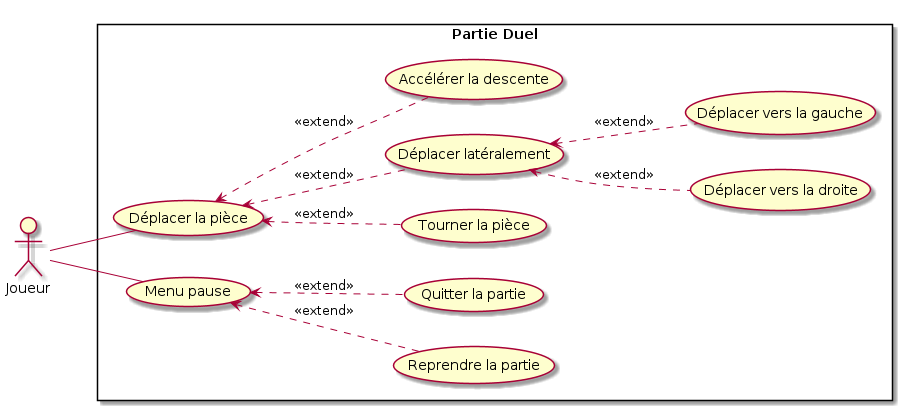
\includegraphics[width=0.9\textwidth]{./uml/usescase/en-jeu/dual.png}
    \caption{Diagramme Use Case en mode Duel}
    \label{fig:Duel}
\end{figure}

\subsubsection*{Déplacer la pièce}
\begin{itemize}
    \item \textbf{Acteur}: Joueur
    \item \textbf{Use case}: Déplacer la pièce
    \item \textbf{Description}: Permet au joueur de déplacer une pièce sur le plateau.
    \item \textbf{Précondition}: Une partie est en cours et le joueur contrôle une pièce.
    \item \textbf{Postcondition}: La pièce est déplacée dans une direction choisie.
    \item \textbf{Cas exceptionnels}: Limite du plateau atteinte, collision avec d'autres pièces.
\end{itemize}

\subsubsection*{Tourner la pièce}
\begin{itemize}
    \item \textbf{Acteur}: Joueur
    \item \textbf{Use case}: Tourner la pièce
    \item \textbf{Description}: Permet au joueur de tourner la pièce dans une direction donnée.
    \item \textbf{Précondition}: Une partie est en cours et une pièce est active.
    \item \textbf{Postcondition}: La pièce est tournée en conséquence.
    \item \textbf{Cas exceptionnels}: La rotation amène la pièce en dehors des limites.
\end{itemize}

\subsubsection*{Envoyer n-1 malus}
\begin{itemize}
    \item \textbf{Acteur}: Joueur
    \item \textbf{Use case}: Envoyer n-1 malus
    \item \textbf{Description}: Envoie une ligne de malus à l'adversaire.
    \item \textbf{Précondition}: Le joueur a complété un nombre spécifique de lignes.
    \item \textbf{Postcondition}: L'adversaire reçoit le malus.
    \item \textbf{Cas exceptionnels}: Échec de l’envoi du malus, conditions de malus non remplies.
\end{itemize}

\subsubsection*{Menu pause}
\begin{itemize}
    \item \textbf{Acteur}: Joueur
    \item \textbf{Use case}: Menu pause
    \item \textbf{Description}: Permet au joueur d'ouvrir le menu de pause.
    \item \textbf{Précondition}: La partie est en cours.
    \item \textbf{Postcondition}: La partie est en pause.
    \item \textbf{Cas exceptionnels}: Aucun.
\end{itemize}

\subsubsection*{Reprendre la partie}
\begin{itemize}
    \item \textbf{Acteur}: Joueur
    \item \textbf{Use case}: Reprendre la partie
    \item \textbf{Description}: Permet de reprendre la partie après une pause.
    \item \textbf{Précondition}: La partie est en pause.
    \item \textbf{Postcondition}: La partie reprend là où elle s'était arrêtée.
    \item \textbf{Cas exceptionnels}: Aucun.
\end{itemize}

\subsubsection*{Quitter la partie}
\begin{itemize}
    \item \textbf{Acteur}: Joueur
    \item \textbf{Use case}: Quitter la partie
    \item \textbf{Description}: Permet au joueur de quitter la partie en cours.
    \item \textbf{Précondition}: La partie est en cours.
    \item \textbf{Postcondition}: Le joueur quitte la partie et retourne au menu principal.
    \item \textbf{Cas exceptionnels}: Aucun.
\end{itemize}

\subsection{En partie Endless}

\begin{figure}
    \centering
    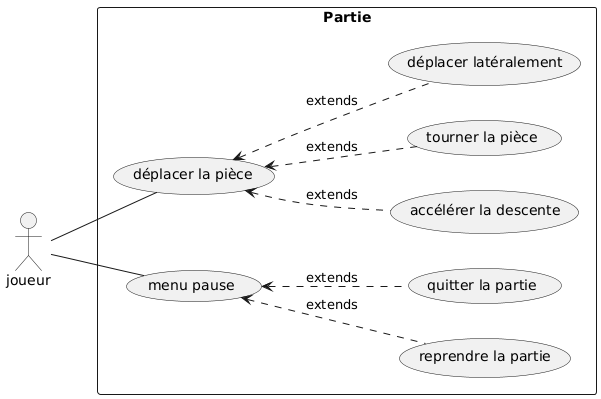
\includegraphics[width=0.9\textwidth]{./uml/usescase/en-jeu/endless.png}
    \caption{Diagramme Use Case en mode Endless}
    \label{fig:Endless}
\end{figure}

\subsubsection*{Déplacer la pièce} (identique à Duel)
\subsubsection*{Tourner la pièce} (identique à Duel)

\subsubsection*{Déplacer latéralement}
\begin{itemize}
    \item \textbf{Acteur}: Joueur
    \item \textbf{Use case}: Déplacer latéralement
    \item \textbf{Description}: Permet au joueur de déplacer la pièce à gauche ou à droite.
    \item \textbf{Précondition}: La pièce est en mouvement.
    \item \textbf{Postcondition}: La pièce est déplacée dans la direction choisie.
    \item \textbf{Cas exceptionnels}: Collision avec d'autres pièces, limite du plateau.
\end{itemize}

\subsubsection*{Accélérer la descente}
\begin{itemize}
    \item \textbf{Acteur}: Joueur
    \item \textbf{Use case}: Accélérer la descente
    \item \textbf{Description}: Permet au joueur d'accélérer la descente de la pièce.
    \item \textbf{Précondition}: Une pièce est en mouvement.
    \item \textbf{Postcondition}: La pièce descend plus rapidement.
    \item \textbf{Cas exceptionnels}: La pièce atteint le bas du plateau plus rapidement que prévu.
\end{itemize}

\subsubsection*{Menu pause} (identique à Duel)
\subsubsection*{Reprendre la partie} (identique à Duel)
\subsubsection*{Quitter la partie} (identique à Duel)

\subsection{En partie Royal Competition}

\begin{figure}
    \centering
    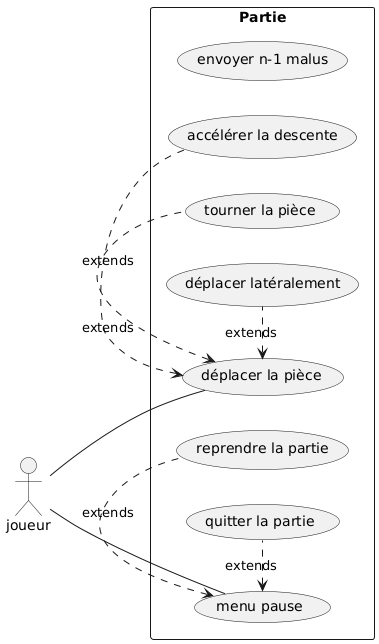
\includegraphics[width=0.9\textwidth]{./uml/usescase/en-jeu/royal-competition.png}
    \caption{Diagramme Use Case en mode Royal Competition}
    \label{fig:Royal-Competition}
\end{figure}

\subsubsection*{Déplacer la pièce} (identique à Duel)
\subsubsection*{Tourner la pièce} (identique à Duel)
\subsubsection*{Envoyer n-1 malus} (identique à Duel)

\subsubsection*{Discuter}
\begin{itemize}
    \item \textbf{Acteur}: Joueur
    \item \textbf{Use case}: Discuter
    \item \textbf{Description}: Permet aux joueurs de discuter entre eux pendant la partie.
    \item \textbf{Précondition}: Une partie multijoueur est en cours.
    \item \textbf{Postcondition}: Message envoyé à l'adversaire.
    \item \textbf{Cas exceptionnels}: Connexion interrompue, messages non envoyés.
\end{itemize}

\subsubsection*{Déplacer latéralement} (identique à Endless)
\subsubsection*{Accélérer la descente} (identique à Endless)
\subsubsection*{Menu pause} (identique à Duel)
\subsubsection*{Reprendre la partie} (identique à Duel)
\subsubsection*{Quitter la partie} (identique à Duel)

\section{Besoin système : Fonctionnels}

\subsection{Connexion}

\subsection{Gestion des comptes}

\subsubsection{Création d'un compte}

\subsubsection{Suppression d'un compte}

\subsection{Consulter le classement}

\subsection{Gestion de la partie}

\subsection{Gestion des amis}

\subsubsection{Gestion du chat}

\subsection{Fin de la partie}

\subsubsection{Fin de la partie normale}

\subsubsection{Fin de la partie Duo}

\subsubsection{Fin de la partie Endless}

\section{Besoins non fonctionnels}

\subsection{Besoins système}

\subsubsection{Réseau}

\subsubsection{Système d'exploitation}

\subsubsection{Accessibilité}

\subsubsection{Performances}

\subsubsection{Capacité}

\subsubsection{Sécurité}

\subsubsection{Robustesse}

\subsection{Besoins utilisateur}

\section{Architecture du système}

\subsection{Architecture du serveur}

\subsection{Architecture du jeu}

\subsection{Architecture du client}

\section{Fonctionnement du système}

\subsection{Création d'un compte}

\subsection{Connexion}

\subsection{Envoie d'une requête}

\subsection{Traitement de la requête}

\subsection{Lancement d'une partie}

\subsection{Rejoindre une partie} 

\end{document}